
\chapter{GIỚI THIỆU TỔNG QUAN}
Chương này cung cấp một cái nhìn tổng quan về nền Công nghiệp 4.0 (Industrie 4.0) - Về kiến trúc của một ứng dụng Công nghiệp 4.0 cũng như các ứng dụng mà các công nghệ trong nền Công nghiệp 4.0 mang lại. Với sự phát triển nhanh chóng của công nghệ điện - điện tử, công nghệ thông tin và công nghệ sản xuất tiên tiến, phương thức sản xuất của các doanh nghiệp sản xuất đang được chuyển từ kỹ thuật số sang thông minh. Và Nhà máy thông minh (Smart Factory) là một giải pháp sản xuất linh hoạt và hiệu quả để đáp ứng được nhu cầu của thị trường ngày nay. Những thuận lợi và thách thức của Nhà máy thông minh cũng sẽ được phân tích trong chương này để chúng ta có thể thấy được tầm quan trọng của nó cũng như những khuyết điểm cần được nghiên cứu và khắc phục.


\section{Tổng quan về Công nghiệp 4.0}

Quá trình công nghiệp hóa bắt đầu với sự ra đời của các thiết bị sản xuất cơ khí vào cuối thế kỷ 18. Sự phát triển động cơ hơi nước của James Watt đã dẫn đến cách mạng hóa cách sản xuất sản phẩm bằng máy móc và động cơ. Bên cạnh đó, xã hội nông nghiệp cũng chuyển thành xã hội công nghiệp. Cho đến nay, bốn cuộc cách mạng công nghiệp đã xảy ra như Hình 1.1. Cuộc cách mạng công nghiệp đầu tiên đã tạo ra những cải tiến vượt bậc nhờ cơ giới hóa, năng lượng hơi nước và khung dệt. Sự chuyển đổi này được theo sau bởi cuộc cách mạng công nghiệp lần thứ hai vào đầu thế kỷ 20 và lần chuyển đổi này liên quan đến sản xuất hàng loạt, dây chuyền lắp ráp và năng lượng điện. Cuộc cách mạng này ngụ ý những thay đổi về tổ chức, chẳng hạn như việc triển khai dây chuyền lắp ráp của Henry Ford và các quy trình quản lý khoa học dựa trên \textit{Frederic W. Taylor}, hay còn được gọi là \textit{Chủ nghĩa Taylor}. Trong cuộc cách mạng này, sản xuất hàng loạt như sản xuất công nghiệp quy mô lớn tăng lên. Do đó, ngành hóa chất và điện tử, cũng như ngành cơ khí và ô tô đã tận dụng những cuộc cách mạng này và bắt đầu phát triển.

\begin{figure}[!h]
    \centering
    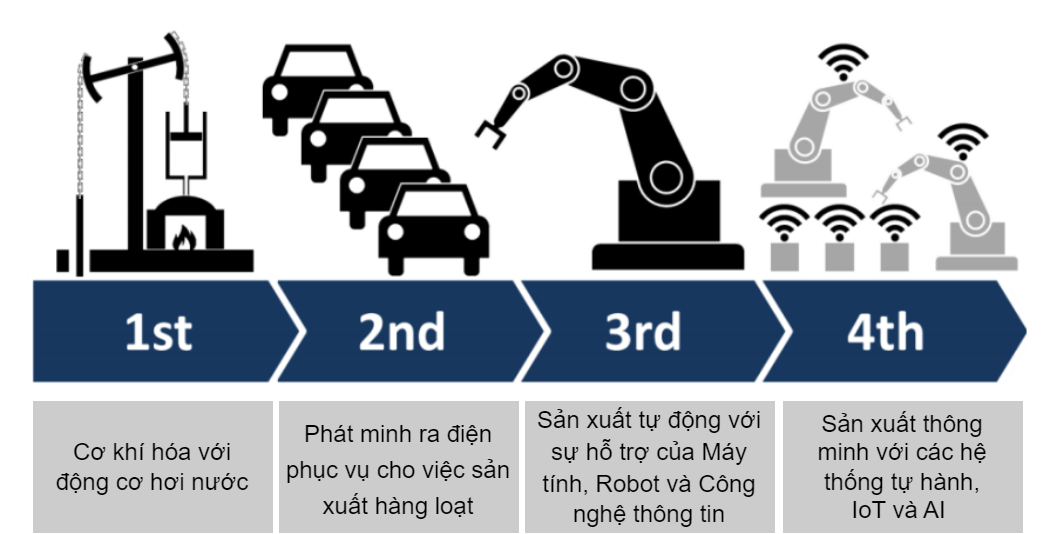
\includegraphics[width=0.9\textwidth]{Images/Intro/4.0revolution.jpg}
    \caption{Các cuộc cách mạng khoa học công nghệ của nhân loại}
    \label{fig:comp_mqtt}
\end{figure}

Vào đầu những năm 1970, cuộc cách mạng công nghiệp lần thứ ba đã xuất hiện và nó vẫn tiếp tục cho đến ngày nay. Ứng dụng điện tử và công nghệ thông tin là những đặc điểm nổi bật nhất của cuộc cách mạng này giúp tăng cường tự động hóa các quy trình sản xuất, cũng như thay thế máy móc thay cho người lao động. Do đó, nó tạo ra nhiều hiệu quả về kinh tế-xã hội và văn hóa-xã hội. Hơn nữa, sản xuất hàng loạt linh hoạt đã tăng năng suất của các quy trình sản xuất. Ngày nay, cuộc cách mạng lần thứ ba vẫn hiện diện nhưng đang chuyển mình uyển chuyển sang một thời đại công nghiệp hóa mới hay còn gọi là cuộc cách mạng công nghiệp lần thứ tư (Industry 4.0). Cuộc cách mạng công nghiệp lần thứ tư đặc trưng bởi việc đưa Internet vạn vật (IoT) vào sản xuất, cho phép các nhà máy thông minh có hệ thống sản xuất tích hợp theo chiều dọc và chiều ngang. Đó là một sự chuyển đổi lớn của toàn bộ ngành sản xuất công nghiệp bằng cách kết hợp các công nghệ kỹ thuật số và internet với ngành công nghiệp truyền thống.

Internet vạn vật, hay còn gọi là Internet of Things – IoTs, là một cuộc cách mạng trong việc kết nối giữa các thiết bị không dây với nhau. Ban đầu, chúng ta có mạng Internet, một thành tựu của cuộc cách mạng khoa học công nghệ lần thứ 3, cho phép các máy tính có thể kết nối và trao đổi thông tin toàn cầu. Tuy nhiên, với sự phát triển nhanh chóng của ngành vi cơ điện tử (Micro Electro Mechanical System), không chỉ máy tính, giờ đây rất nhiều các thiết bị có khả năng kết nối vào mạng Internet. Thông dụng nhất trong cuộc sống mà chúng ta có thể kể đến như các điện thoại thông minh, máy tính bảng, các loại thẻ thông minh (Smart cards) hay như các nốt trong mạng cảm biến không dây (Wireless Sensor Networks). Với những đặc tính đó, một thế hệ mạng mới đã được hình thành, và là sản phẩm đặc trưng cho cuộc cách mạng khoa học công nghệ lần thứ 4, mạng Internet vạn vật, hay còn gọi là IoT - Internet of Things.

Dựa trên mạng Internet vạn vật, các ứng dụng không còn ở khái niệm thông minh nữa, mà sẽ tiến lên một bước cao hơn, gọi là tự hành (autonomous), chẳng hạn như các ứng dụng giám sát và tự động thích nghi trong việc điền khiển như các dịch vụ trong nhà, bãi giữ xe, hay các hệ thống quan trắc trong nông nghiệp, thủy hải sản. Theo diễn giả nổi tiếng Timothy Chou, kiến trúc của các ứng dụng thời đại cách mạng công nghiệp 4.0 dựa trên Internet vạn vật nói chung và sản xuất thông minh trong công nghiệp nói riêng, được chia thành mô hình 5 lớp, như mô tả ở hình bên dưới.

\begin{figure}[!h]
    \centering
    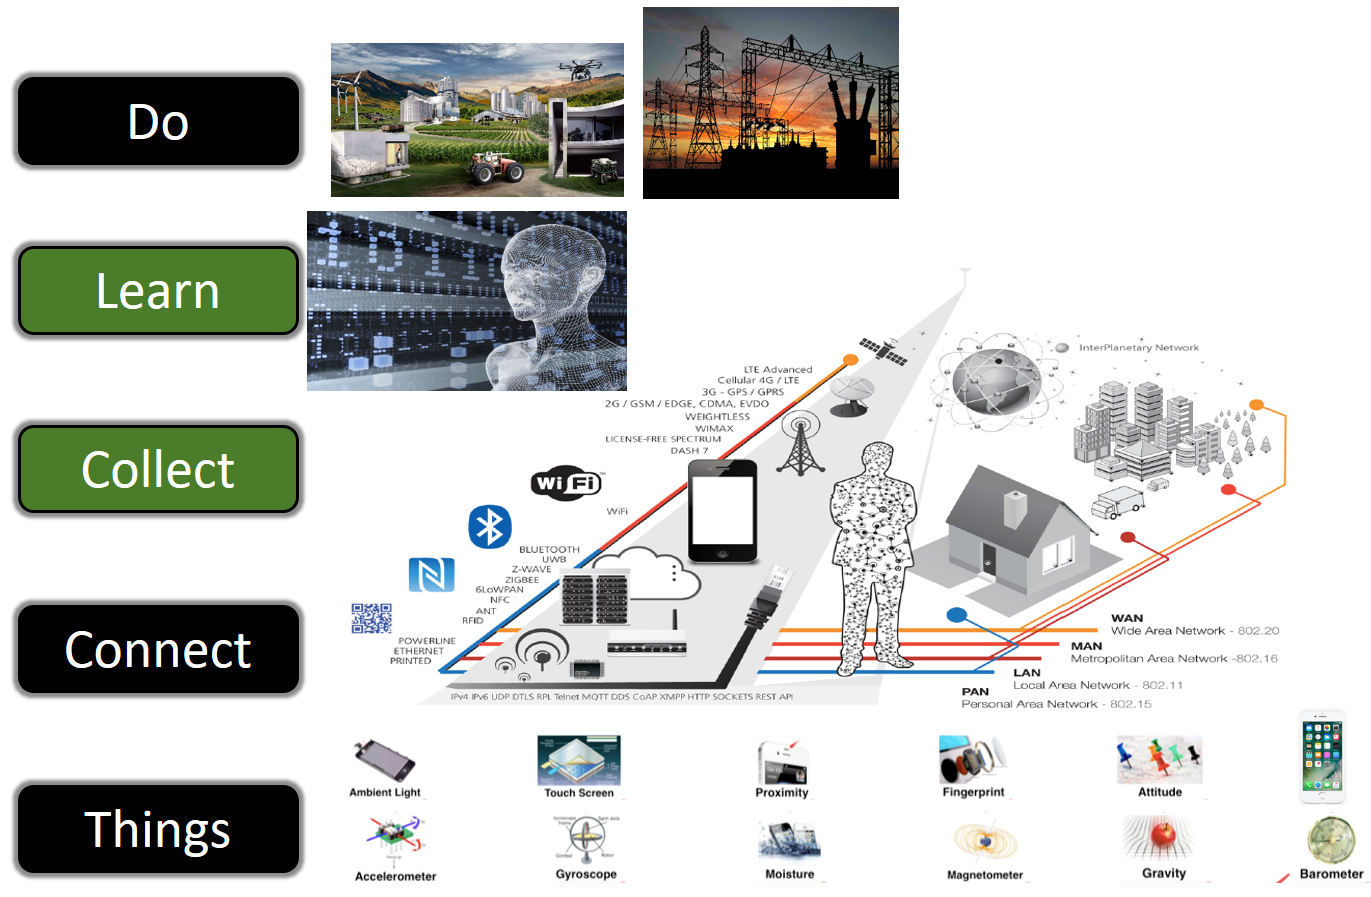
\includegraphics[width=\textwidth]{Images/Intro/5layer.jpg}
    \caption{Kiến trúc chung cho các ứng dụng thời đại 4.0 \cite{iotp}}
    \label{fig:comp_mqtt}
\end{figure}

Lớp đầu tiên bao gồm các Things. Things ở đây chính các máy móc và chúng được kết nối với Internet theo nhiều cách khác nhau. Sau khi được kết nối, Lớp Collect ở đây đề cập đến các công nghệ được thiết kế để thu thập dữ liệu - dữ liệu chuỗi thời gian được gửi đi mỗi giờ, phút hoặc giây. Lớp thứ tư là Learn. Không giống như trong thế giới của các ứng dụng IoP (Internet of People), nơi chúng ta phải nhập những nội dung input nào đó, thì các ứng dụng IoT sẽ lấy dữ liệu một cách liên tục. Ví dụ, chúng ta có thể sử dụng máy móc để học hỏi (learn) từ những Things của mình tại bệnh viện, hầm mỏ hoặc trang trại. Và cuối cùng, chúng ta sẽ có những câu hỏi, Những công nghệ này để làm gì? Kết quả kinh doanh là gì? Thì khi đó, Lớp Do mô tả cả công nghệ ứng dụng phần mềm và mô hình kinh doanh bị ảnh hưởng bởi các công ty sản xuất ra Things, cũng như những người sử dụng chúng để cung cấp dịch vụ chăm sóc sức khỏe, vận chuyển hoặc xây dựng chẳng hạn. Và chức năng chính của từng lớp trong kiến trúc này được khái quát như sau:
\begin{itemize}
    \item \textbf{Things}: Các thiết bị trong ứng dụng giám sát. Chúng ta có thể thấy, đây là lớp rất phong phú về mặt số lượng và đa dạng về chức năng. Rất nhiều các loại cảm biến sẽ được dùng, tùy vào các ứng dụng giám sát. Bên cạnh đó, các nốt cảm biến sẽ chủ yếu dựa vào giao tiếp không dây
    \item \textbf{Connect}: Thu thập dữ liệu từ các nốt cảm biến. Do có rất nhiều tiêu chuẩn kết nối tùy theo từng loại ứng dụng, lớp này phải hỗ trợ nhiều loại kết nối, từ giao tiếp Zigbee và Wifi trong các ứng dụng nhà thông minh, với khoảng cách giao tiếp ngắn cho đến các giao trên không gian rộng như LoRa hay 3G/4G.
    \item \textbf{Collect}: Sau khi dữ liệu được thu thập, chúng sẽ được gửi lên các server tập trung để lưu trữ dữ liệu. Tại đây, một lượng lớn dữ liệu sẽ được đẩy về, tạo ra một thách thức không nhỏ cho các server và phải ứng dụng các công nghệ về Big Data (dữ liệu lớn) để xử lý.
    \item \textbf{Learn}: Nhiệm vụ của lớp này là lọc ra các thông tin đặc trưng, có ngữ nghĩa đặc thù cho từng loại ứng dụng. Các công nghệ về Học Máy và hiện tại là Học Sâu (Deep Learning) sẽ được áp dụng ở đây.
    \item \textbf{Do}: Dựa vào các thông tin đặc trưng, hệ thống sẽ xây dựng nên những quy luật thích nghi theo ngoại cảnh, và đề xuất các quyết định cho hệ thống. Với mỗi quyết định, việc thực thi sẽ được đo đạc một cách tự động, và sai lệnh của quyết định đó so với mục tiêu tối ưu sẽ được xem xét lại cho lần sau. Theo cách này, hệ thống sẽ tự động tích lũy “kinh nghiệm” trong một thời gian dài, để ngày càng trở nên thông minh và hoàn thiện hơn.
    
\end{itemize}

Sự phát triển mạnh mẽ của khoa học công nghệ ở những năm đầu thế kỉ 21 đã đưa nhân loại bước vào cách mạng công nghiệp 4.0, khi mà "hàng tỉ" thiết bị có thể giao tiếp và chia sẻ dữ liệu với nhau thông qua mạng kết nối vạn vật (Internet of Things). Theo ước tính của cộng đồng khoa học, đến năm 2025 sẽ có 75 tỉ thiết bị có thể kết nối mạng Internet với nhau. Và với sự bùng nổ về số lượng thiết bị kết nối đó, vô tình mang lại một trọng trách lớn đối với Lớp Connect - trong đó, các giao thức truyền thông đóng một vai trò đặc biệt quan trọng để có thể giúp các thiết bị kết nối và giao tiếp với nhau một cách hiệu quả.

% Cuộc cách mạng công nghiệp lần thứ tư đặc trưng bởi việc đưa Internet vạn vật (IoT) vào sản xuất, cho phép các nhà máy thông minh có hệ thống sản xuất tích hợp theo chiều dọc và chiều ngang.  Các công ty đang phải đối mặt với nhiều thách thức trong việc triển khai Công nghiệp 4.0. Để giảm thiểu những thách thức này và cấu trúc Công nghiệp 4.0, đã có những sáng kiến phát triển các mô hình kiến trúc tham chiếu trừu tượng. Và với Đồ án này, chúng em sẽ sử dụng mô hình kiến trúc tham chiếu được phát triển bởi Nền tảng công nghiệp 4.0 của Đức (RAMI 4.0) để nghiên cứu về các lớp trong kiến trúc của một ứng dụng trong nền Công nghiệp 4.0. 

% \subsection{Kiến trúc của ứng dụng trong thời đại 4.0}

% \begin{figure}[!h]
%     \centering
%     \includegraphics[width=0.7\textwidth]{Images/Intro/layers.jpg}
%     \caption{Sự phân chia thế giới thông tin/thế giới vật lý và sự phù hợp của Công nghiệp 4.0 trong RAMI 4.0}
%     \label{fig:comp_mqtt}
% \end{figure}

% \subsubsection{Lớp Asset và Lớp Integration}
% Nội dung số dưới dạng dữ liệu và chức năng được tiêu chuẩn hóa, và kết nối kỹ thuật số dựa trên quy tắc của thế giới vật lý (physical world) với thế giới thông tin (information world) là những yếu tố quyết định sự thành công của các mô hình kinh doanh mới.\\
% Lớp Asset tạo thành cấp thấp nhất trong RAMI 4.0. Nó phản ánh thế giới vật lý. Năm lớp trên nó thì được liên kết với thế giới thông tin.\\
% Lớp Integration kết nối thế giới vật lý của một asset và thế giới thông tin của Công nghiệp 4.0 (Industrie 4.0). Nó có thể được coi là một loại dịch giả giữa hai thế giới. Để lấy ví dụ, ta đưa nó vào bối cảnh: Việc tạo ra phép đo kỹ thuật số dựa trên giá trị vật lý diễn ra ở cấp độ này bằng một máy biến áp tương tự sang kỹ thuật số (analogue-to-digital). Hoặc ta xem xét theo một hướng khác: một lệnh vị trí ảo (virtual position command) được chuyển đổi thành giá trị tương tự (analogue) để nó có thể thiết lập một vị trí van, ... Hơn nữa, Lớp Integration là lớp kết hợp các công nghệ hiện được công nhận là thuộc về nền Công nghiệp 3.x (Industrie 3.x). Còn thế giới Công nghiệp 4.0 được căn chỉnh ở năm cấp độ cao hơn.\\
% Điều này có nghĩa là:
% \begin{itemize}
%     \item Các công nghệ của nền Công nghiệp 3.x (Industrie 3.x) nằm trong Lớp Integration 
%     \item Tất cả nội dung của Industrie 4.0-compliant có thể được quy cho một trong bốn cấp độ cao hơn
% \end{itemize}
% Lớp Integration chứa:
% \begin{itemize}
%     \item Thông tin về các yêu cầu và trạng thái thay đổi trong suốt quá trình gia tăng giá trị trong thế giới vật lý. Những thay đổi điển hình là những thay đổi như thay đổi trạng thái của một khối tổng thể (ví dụ: độ đặc của chất kết dính thay đổi từ lỏng sang rắn) hoặc thay đổi vật liệu do quá trình xử lý (ví dụ: phôi gia công được làm nóng và điều này làm thay đổi độ bền của nó). Những sự kiện xảy ra trong thế giới vật lý này phải được xác định trong Lớp Integration - ít nhất là ở dạng thông tin (đã thay đổi).
%     \item Dữ liệu, chức năng và ứng dụng dành riêng cho nhà sản xuất và không tuân thủ Công nghiệp 4.0 vì nhà sản xuất muốn bảo vệ (và không chia sẻ) kiến thức của họ.
%     \item Những asset liên quan chặt chẽ hoặc có liên quan đến thế giới thông tin, chẳng hạn như hệ điều hành, firmware hoặc runtime framework.
% \end{itemize}
% Đồng thời, nó còn áp dụng những điều sau:
% \begin{itemize}
%     \item Mỗi "điểm thông tin" quan trọng (information point) (tức là một sự kiện) trong thế giới vật lý đều tạo ra một điểm thông tin trong thế giới thông tin, ít nhất là trong Lớp Integration.
%     \item Nếu các điểm thông tin này tuân thủ Công nghiệp 4.0 thì chúng sẽ được xử lý ở các lớp cao hơn.
%     \item Mặt khác, với mọi điểm thông tin trong thế giới thông tin, không nhất thiết phải có một điểm thông tin tương ứng trong thế giới vật chất. Một ví dụ về điều này sẽ là những asset đã được hủy bỏ nhưng vẫn nằm trong kho lưu trữ của thế giới thông tin, hoặc có lẽ chúng chưa từng tồn tại trong thực tế và chỉ hiện diện trong thế giới thông tin với mục đích mô phỏng.
% \end{itemize}
% Quá trình chuyển đổi từ Industrie 3.x sang Industrie 4.0 diễn ra khi tất cả dữ liệu, chức năng, hệ thống truyền thông, v.v. thuộc Lớp Integration nhưng không tương thích với Industrie 4.0 dần dần được thay thế bằng các bản sao phù hợp và sau đó có thể được định vị trong những lớp cao hơn có liên quan.\\
% Như vậy, tất cả các nhà máy hiện có đều có khả năng từng bước được nâng cấp để phù hợp với Industrie 4.0. Các nhà máy có thể tự cung cấp dữ liệu mới ban đầu và những chức năng cho Công nghiệp 4.0 hoặc họ có thể sử dụng giải pháp "gateway" bằng phần cứng bổ sung để thu thập dữ liệu và chức năng từ các nhà máy đã tồn tại trong mạng Công nghiệp 4.0.\\
% Do đó, Lớp Integration đóng vai trò chính trong việc tạo điều kiện thuận lợi cho sự chuyển đổi từ Công nghiệp 3.x sang Công nghiệp 4.0.\\
% Mặc dù tỷ lệ các giải pháp Công nghiệp 4.0 mở (open Industrie 4.0) sẽ tiếp tục tăng, nhưng sẽ luôn có một tỷ lệ nhất định vẫn thuộc sở hữu độc quyền. Lớp Integration sẽ đóng vai trò trung tâm trong vấn đề này trong tương lai.

% \subsubsection{Lớp Communication}
% Trong Công nghiệp 4.0, mạng all-encompassing và các tương tác (interactions) xa hơn nhiều so với trước đây. Mục đích là để có khả năng plug-and-play, minh bạch trên tất cả các cấp độ phân cấp và hỗ trợ các dịch vụ mới nhất. Đối với điều này, các giải pháp từ các lĩnh vực truyền thông công nghiệp (industrial communication) và công nghệ thông tin phải được kết hợp với nhau. Mục tiêu là mọi asset có thể trao đổi thông tin với mọi asset khác trong mạng, bất kể cấp độ tương ứng của chúng trong hệ thống phân cấp.\\
% Lớp Communication bao gồm các khả năng chẳng hạn như sự giao dịch tự động (autonomous negotiation) diễn ra giữa các asset khi thiết lập kết nối giao tiếp, về bit rates, chất lượng truyền và bảo mật trong số những thứ khác. Lớp này đảm nhận việc vận chuyển dữ liệu an toàn và đúng giờ trên cơ sở kiến trúc hướng dịch vụ, thậm chí vượt ra ngoài ranh giới công ty.\\
% "Communication" trong ngữ cảnh này chỉ có nghĩa là sự chuyển giao giữa hai bên tham gia. Nội dung truyền tải, chẳng hạn như dữ liệu được định vị và mô tả trong Lớp thông tin. Giao diện giao tiếp (communication interface) của một asset được mô tả trong Lớp Communication và từ quan điểm của interface user (của asset), giao tiếp đại diện cho một chủ đề (subject).

% \subsubsection{Lớp Information}
% Lớp này cung cấp quá trình xử lý trước các sự kiện và thực thi các quy tắc liên quan đến sự kiện bằng cách cho phép mô tả chính thức của chúng để giải thích thông tin. Nó cũng quản lý tính liên tục của dữ liệu, đảm bảo tính toàn vẹn và chuyển đổi dữ liệu nhất quán để đưa vào Lớp Functional. Do đó, nó bao gồm cảm biến và xử lý trước dữ liệu kế thừa trong khi đưa vào môi trường Xử lý Dòng và Xử lý Hàng loạt tương ứng. Cuối cùng, lớp này cũng bao gồm DB của nền tảng bảo trì dự đoán và DB chuỗi thời gian cho các phép đo cảm biến theo thời gian thực. Bằng cách này, dữ liệu yêu cầu được trích xuất và kết hợp tương ứng để có sẵn bởi các chức năng của lớp tiếp theo. Quá trình này cũng tuân theo Thu thập dữ liệu và Thao tác Dữ liệu của tiêu chuẩn ISO 13374 do MIMOSA OSA-CBM thực hiện.

% \subsubsection{Lớp Functional}
% Lớp Functional bao gồm tất cả các chức năng và dịch vụ tuân thủ các quy ước của Công nghiệp 4.0. Chúng lấy thông tin của chúng từ dữ liệu I4.0 trong Lớp Information và gửi kết quả tới Lớp Information và các lớp tiềm năng khác, cũng ở dạng dữ liệu I4.0. Mục tiêu là mọi asset có thể hợp tác với mọi asset khác trong mạng.\\
% Trong Lớp Functional, có một sự khác biệt được tạo ra giữa các chức năng cơ bản (basic functions), chức năng quy trình (process functions) và chức năng dành riêng cho nhà sản xuất (manufacturer-specific functions).\\

% \textbf{Chức năng cơ bản (Basic functions)}\\
% Một chức năng cơ bản là một chức năng thường có sẵn và phù hợp với I4.0. Một ví dụ là chức năng "giám sát tình trạng" (condition monitoring) cho các thành phần của máy. Chức năng cơ bản này không dành riêng cho nhà sản xuất. Chức năng này yêu cầu dữ liệu chẩn đoán được lưu trữ trong Lớp Information bằng cách sử dụng một định dạng và ngữ nghĩa hài hòa, tuân thủ I4.0 (harmonized, I4.0-compliant format and semantics). Loại giám sát tình trạng này, được hình thành là không dành riêng cho nhà sản xuất hoặc người dùng, được mô tả cùng với dữ liệu liên quan trong quy tắc kỹ thuật VDMA 24582, sau đó được đệ trình lên IEC để tiêu chuẩn hóa. Một ví dụ khác về chức năng cơ bản là chức năng drive tuân thủ I4.0. \\

% \textbf{Chức năng quy trình (process functions)}\\
% Các chức năng I4.0 cũng có thể là các chức năng quy trình phục vụ các mục đích của quy trình sản xuất hoặc quy trình công nghệ. Trong trường hợp này, chức năng quy trình thu thập các hướng dẫn quy trình từ Lớp Business đồng thời thu thập dữ liệu và thông tin cần thiết để chức năng được thực hiện từ các lớp bên dưới. Các chức năng này phải có sẵn miễn phí, được mô tả chính thức (trong các tiêu chuẩn) và các chức năng tuân thủ I4.0, chẳng hạn như các chức năng được áp dụng trong công nghệ sản xuất (xem DIN 8580):
% \begin{itemize}
%     \item hình thành sơ cấp (tạo sự gắn kết) (primary forming (creating cohesion))
%     \item cải cách (duy trì sự gắn kết) (reforming)
%     \item tách (giảm sự gắn kết) (separating)
%     \item nối (tăng tính gắn kết) - phủ (tăng tính gắn kết) (joining - coating)
%     \item thay đổi tính chất vật liệu (changing material properties) 
% \end{itemize}
% Chúng cũng đi kèm với các chức năng con, chẳng hạn như với các phương pháp phân tách:
% \begin{itemize}
%     \item loại bỏ (removing) (DIN 8590), ví dụ: cắt nhiệt, cắt plasma hoặc gia công phóng điện…
%     \item làm sạch (cleaning) (DIN 8592)
%     \item loại bỏ chip bằng các lưỡi dao được xác định về mặt hình học (DIN 8589-0), ví dụ: tiện, phay và khoan, v.v.
%     \item loại bỏ chip bằng các lưỡi cắt không xác định về mặt hình học (DIN 8589-0), ví dụ: mài
%     \item tháo rời (disassembling) (DIN 8591)
%     \item cắt đứt (severing) (DIN 8588)
% \end{itemize}
% Các chức năng "truyền thống" cũng được tính là các chức năng tuân thủ I4.0 (I4.0-compliant functions), chẳng hạn như:
% \begin{itemize}
%     \item đo lường (measuring)
%     \item kiểm soát (controlling)
%     \item điều hòa (regulating)
%     \item và những chức năng khác.
% \end{itemize}
% Dự định trong tương lai là một cấu hình asset sẽ có thể tự quyết định quy trình nào cho chính nó, chẳng hạn như loại bỏ chip, sẽ là tốt nhất và tiết kiệm nhất - dựa trên các tùy chọn của nó. Một ví dụ sẽ giúp làm cho điều này rõ ràng hơn. Đơn đặt hàng của khách hàng đi từ Lớp Business đến Lớp Functional (hoặc đến Lớp Information liên quan đến dữ liệu). Nội dung của nó là: Một lỗ có đường kính xác định sẽ được khoan vào kim loại với dung sai không được vượt quá x\%. Sau đó, Lớp Functional xác định "khoan" thực sự có nghĩa là gì, theo các thông số liên quan của nó. Sau đó, nó sử dụng thông tin trong các lớp bên dưới để kiểm tra xem nhà máy (cũng là asset) có sẵn tài nguyên phù hợp ("máy móc") có thể tạo lỗ theo thông số kỹ thuật được yêu cầu hay không. Điều quan trọng cần lưu ý là đây không nhất thiết phải là máy khoan. Tùy thuộc vào hướng dẫn, nó có thể là máy cắt laser, máy ép hoặc máy phay. Nếu nguồn lực cần thiết có sẵn và nếu chi phí nằm trong phạm vi được chỉ định trong Lớp Business, thì đơn đặt hàng có thể đạt được về mặt kỹ thuật và công việc có thể được bắt đầu.\\

% \textbf{Các chức năng dành riêng cho nhà sản xuất (manufacturer-specific functions)}\\
% Ngoài các chức năng không dành riêng cho nhà sản xuất, có thể có các chức năng liên quan đến từng nhà sản xuất hoặc người dùng để tạo ra các đặc tính độc nhất (USPS).

% \subsubsection{Lớp Business}
% Lớp Business mô tả các quy trình business và điều kiện khuôn khổ kinh doanh (business framework conditions) cho asset.\\
% Quy trình business bao gồm tất cả các framework conditions không liên quan ngay đến chức năng kỹ thuật của asset. Đây có thể là việc tự động ký kết hợp đồng điện tử (electronic contracts) giữa các asset, khuôn khổ pháp lý (legal framework) được xây dựng chính thức, chứng chỉ điện tử (electronic certificates), v.v. Dữ liệu Standardized I4.0 được bàn luận ở đây áp dụng cho các quy trình business nhưng trên thực tế có thể thuộc Lớp Information. Chúng bao gồm: Thời gian Switch-on, thời hạn sử dụng, license key, phân quyền hoặc bất kỳ dữ liệu nào liên quan đến việc triển khai các mô hình kinh doanh mới.\\
% Sau đây là các yếu tố quyết định đối với Lớp Business và được mô tả trong DIN SPEC 91345 và IEC PAS 68033:
% \begin{itemize}
%     \item các điều kiện chung về ranh giới của tổ chức (general organizational boundary conditions) (chẳng hạn như vận hành đơn đặt hàng, các điều kiện đặt hàng chung hoặc các quy định pháp lý); điều phối các dịch vụ trên lớp "functional";
%     \item điều kiện tiền tệ (giá cả, nguồn lực sẵn có, chiết khấu, v.v.); đảm bảo tính toàn vẹn của các chức năng trong chuỗi giá trị gia tăng;
%     \item các quy tắc mô hình hóa mà hệ thống I4.0 phải tuân theo;
%     \item lập bản đồ các mô hình business và các quá trình business kết quả; các điều kiện pháp lý và quy định chung;
%     \item liên kết giữa các quy trình kinh doanh khác nhau;
%     \item tiếp nhận các sự kiện để quy trình business chuyển sang giai đoạn tiếp theo.
% \end{itemize}
% \subsection{Ví dụ}

% Ví dụ về trục thủy lực servo sử dụng các lớp kiến trúc của RAMI 4.0\\
% \begin{figure}[!h]
%     \centering
%     \includegraphics[width=\textwidth]{Images/Intro/Example.jpg}
%     \caption{Trục thủy lực servo sử dụng kiến trúc RAMI 4.0}
%     \label{fig:comp_mqtt}
% \end{figure}

% Ví dụ sau (Hình 1.2) mô tả sự phân bố chức năng trên các lớp khác nhau của RAMI 4.0.\\
% Trục servo-thủy lực là một hệ thống bao gồm một số thành phần. Trong trường hợp này, asset là những thứ như xi lanh thủy lực, những khối có bơm tích hợp và động cơ servo. Bộ tăng cường ổ đĩa (drive enhancer) - cũng là một asset - được kết nối qua cáp. Nó tạo ra một kết nối với động cơ servo điện, có nghĩa là phần cứng của nó được phân bổ cho Lớp asset và bản sao kỹ thuật số (digital counterpart) của nó nằm trong Lớp Integration. Các chức năng độc quyền như bộ điều chỉnh mô-men xoắn và bộ điều tốc cũng được định vị trong Lớp Integration, cũng như dữ liệu liên quan. Nên giả định rằng tồn tại một 
% chức năng tuân thủ I4.0 có thể xác định hiệu quả năng lượng bằng cách sử dụng dữ liệu tuân thủ I4.0. Kiểm soát vị trí cũng phải tuân theo I4.0 và nó phải sử dụng dữ liệu tuân thủ I4.0. Những dữ liệu này được truyền qua giao diện truyền (communication interface) thông phù hợp với I4.0 (ví dụ cáp Ethernet OPC-UA, v.v.) và có sẵn dưới dạng dữ liệu I4.0 trong Lớp Information. Quy trình business của Lớp Business bao gồm quản lý năng lượng tuân thủ I4.0 (ví dụ: phù hợp với ISO 50001). Sau khi đánh giá dữ liệu năng lượng thô, hệ thống quản lý năng lượng sử dụng chức năng liên quan trong Lớp Functional để truy cập dữ liệu được tạo trong Lớp Integration.\\
% Bộ điều chỉnh vị trí cũng là một asset. Nó được biểu diễn theo RAMI 4.0 và được liên kết với điều khiển đầu (head control). Thực tế, điều này có nghĩa là nó nhận các lệnh vị trí (position instructions) từ RAMI 4.0 của bộ điều khiển đầu (nhận được thông qua giao tiếp tuân thủ I4.0) và sử dụng các lệnh này cho quy định vị trí của riêng nó.\\
% Sự chuyển đổi của công nghệ hiện tại sang Industrie 4.0 có thể dễ dàng nhận thấy trong ví dụ này. Nó cũng cho thấy rằng có thể bắt đầu với dữ liệu tuân thủ Industrie 4.0 bị hạn chế và dần dần các dữ liệu và chức năng khác có thể được giới thiệu phù hợp với I4.0.\\

\section{Các công nghệ Công nghiệp 4.0}

Ứng dụng công nghệ Công nghiệp 4.0 bao gồm các công nghệ khác nhau như Internet vạn vật (IoT), điện toán đám mây, additive manufacturing, an ninh mạng với blockchain, augmented reality với trí tuệ nhân tạo (AI), big data, tích hợp hệ thống (system integration), mô phỏng (simulation), robot tự hành và \textbf{digital twin}. Nhiều công nghệ trong số này đã được sử dụng trong sản xuất, nhưng với ngành công nghiệp 4.0, chúng sẽ chuyển đổi thành quy trình sản xuất dưới dạng các cell được tối ưu hóa sẽ kết hợp với nhau thành một quy trình sản xuất được tích hợp hoàn toàn, tự động hóa và tối ưu hóa. Chúng làm tăng hiệu quả và thay đổi hệ thống chuỗi cung ứng truyền thống, cũng như mối quan hệ giữa con người và máy móc. Các kỹ thuật của Công nghiệp 4.0 có khả năng cải thiện việc sử dụng năng lượng, thiết bị và nguồn nhân lực. Công nghiệp 4.0 là một cấu trúc tương lai nuôi dưỡng sự phát triển của các hệ thống sản xuất tự trị với ứng dụng IoT, CPS và AI. Các công nghệ dựa trên cảm biến mới giúp các doanh nghiệp vừa và nhỏ theo dõi liên tục việc sử dụng máy móc, nhu cầu năng lượng và đào tạo nhân viên. Bằng cách phân tích kỹ lưỡng các công nghệ Công nghiệp 4.0 khác nhau, dữ liệu từ các thiết bị IoT khác nhau có thể được xử lý để cải thiện tính bền vững của hoạt động sản xuất.

\begin{figure}[!h]
    \centering
    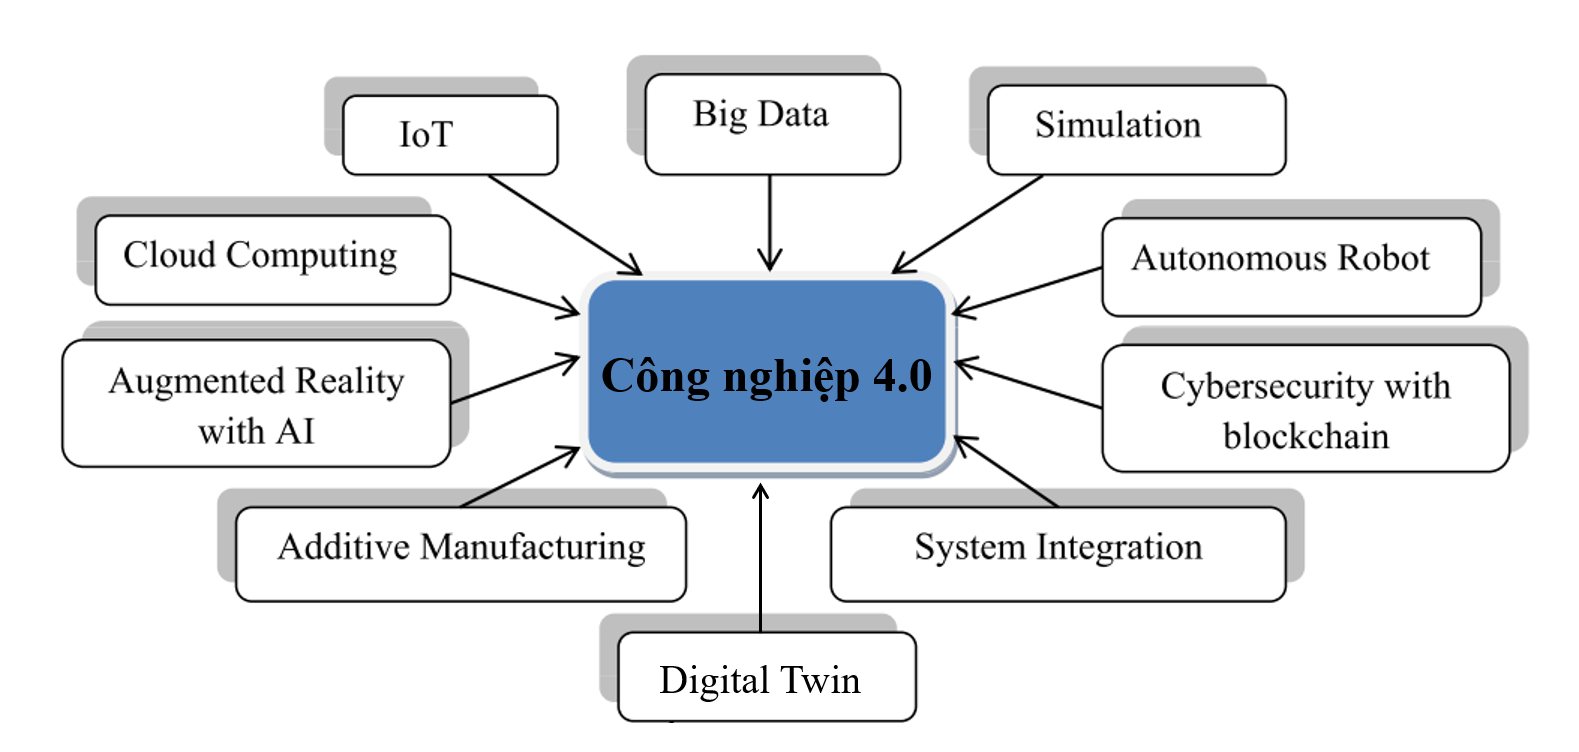
\includegraphics[width=\textwidth]{Images/Intro/4.0appliction.jpg}
    \caption{Các công nghệ của Công nghiệp 4.0}
    \label{fig:0appliction}
\end{figure}

% Để hoạt động bền vững, các sản phẩm cần được sản xuất theo quy trình thân thiện với môi trường, khả thi về mặt xã hội và hiệu quả kinh tế. Các hệ thống sản xuất dựa trên các quy trình sản xuất có đạo đức và bền vững có hiệu quả cao trong việc tiết kiệm năng lượng và tài nguyên thiên nhiên. Công nghiệp 4.0 là một cấu trúc xã hội kỹ thuật trong đó các triển vọng về công nghệ, xã hội và tổ chức tương tác với nhau. Kết nối bền vững với Công nghiệp 4.0 cần được nghiên cứu sâu. Để tiết kiệm năng lượng, giảm phế liệu và tác động của nó đối với môi trường, chuỗi giá trị công nghiệp phải được định hướng theo hướng bền vững. 

Các công nghệ này có thể đóng góp đáng kể cho sự bền vững bằng cách giảm lượng khí thải carbon, sử dụng năng lượng tái tạo và các giải pháp công nghệ phù hợp cho cả cá nhân và xã hội. Sự phát triển của Công nghiệp 4.0 giúp sử dụng tối ưu các nguồn tài nguyên theo cách minh bạch hơn. Bằng cách thực hiện các phương pháp của Công nghiệp 4.0, hiệu quả sản xuất và đổi mới có thể được cải thiện, ảnh hưởng đến tính bền vững về xã hội và môi trường. Có nhiều lợi ích được đóng góp riêng bởi các công nghệ khác nhau của Công nghiệp 4.0. Các ứng dụng quan trọng của các công nghệ Công nghiệp 4.0 này được tóm tắt trong Bảng 1.1


\begin{longtblr}[
caption = {Ứng dụng của các công nghệ Công nghiệp 4.0},
label = {tblr:my-table},
entry = {Ứng dụng của các công nghệ Công nghiệp 4.0}
]{
hlines,vlines,
colspec = {X[2,c]X[3,j]},
columns = {valign = m},
}
\centering\textbf{Các công nghệ của Công nghiệp 4.0} &
  \textbf{Ứng dụng} \\ 
IoTs &
  IoT tích hợp các cảm biến vào hệ thống sản xuất. Các cảm biến và máy móc của nhà sản xuất được kết nối mạng và sử dụng điện toán nhúng. Nó tạo ra khả năng thu thập và phân tích dữ liệu theo cách phi tập trung. \\ 
{Điện toán đám mây \\ (Cloud computing)} &
  Truy cập dữ liệu có sẵn mọi lúc mọi nơi; tính minh bạch và khả năng đáp ứng của chuỗi cung ứng; dễ dàng chia sẻ dữ liệu quan trọng; hỗ trợ từ các đối tác trong chuỗi cung ứng trong việc nâng cấp công nghệ, dữ liệu về vòng đời sản phẩm có thể được lưu trữ và truy xuất theo triết lý CE. \\ 
Augmented Reality &
 Các hệ thống dựa trên Augmented Reality hỗ trợ nhiều dịch vụ khác nhau, chẳng hạn như chọn các bộ phận trong kho và gửi hướng dẫn sửa chữa qua thiết bị di động. Nó cung cấp thông tin theo thời gian thực để giúp các nhà sản xuất đưa ra quyết định theo thời gian thực và cải thiện quy trình làm việc.\\
{Sản xuất phụ gia \\ (Additive manufacturing - AM)} &
  Sản xuất phụ gia hoặc in 3D được sử dụng để sản xuất các lô sản xuất nhỏ theo yêu cầu. Nó tạo ra những lợi thế như là: sản xuất các sản phẩm phức tạp và cấu trúc nhẹ. Hệ thống AM phi tập trung và hiệu suất cao này sẽ giảm khoảng cách vận chuyển và lượng hàng tồn kho. Do đó, nó sửa đổi hệ thống chuỗi cung ứng. \\ 
{Tích hợp hệ thống \\ (System integration)} &
 Trong ngành công nghiệp 4.0, các công ty, bộ phận, phòng ban, chức năng sẽ trở nên gắn kết hơn nhiều, với tư cách là cross-company. Do đó, cross-company này, cũng như các mạng tích hợp dữ liệu toàn cầu phát triển và cho phép các chuỗi giá trị thực sự tự động. Do đó, nó tạo ra sự kết nối trong chuỗi cung ứng, giữa nhà cung cấp và khách hàng thông qua tích hợp theo chiều ngàg và dọc.\\
{An ninh mạng \\ (Cyber-security)} &
 Công nghiệp 4.0 làm tăng khả năng kết nối và sử dụng các giao thức truyền thông tiêu chuẩn. Khi đó, cần phải bảo vệ các hệ thống thông tin, hệ thống công nghiệp, dây chuyền sản xuất và thiết bị khỏi các mối đe dọa an ninh mạng với tần suất ngày càng tăng cao. Điều cần thiết là tạo ra thông tin liên lạc an toàn, đáng tin cậy, cũng như quản lý truy cập và nhận dạng tinh vi của máy móc và người dùng.\\
Robot tự hành &
  Ngày nay, robot được sử dụng để giải quyết các nhiệm vụ phức tạp và cộng tác với nhau và với con người. Những robot này tự chủ, linh hoạt và hợp tác. Hơn nữa, chúng có chi phí thấp hơn và có nhiều khả năng hơn so trước đây.\\
{Mô phỏng \\ (Simulation)} &
 Mô phỏng 2D hoặc 3D của quá trình phát triển sản phẩm, phát triển vật liệu và sản xuất đã được sử dụng trong thế giới công nghiệp. Ngày nay, mô phỏng phải được sử dụng rộng rãi hơn trong các hoạt động của nhà máy. Những mô phỏng này cung cấp dữ liệu thời gian thực để phản ánh thế giới thực trong một mô hình ảo, bao gồm máy móc, sản phẩm và con người. Nó giúp làm giảm thời gian thiết lập máy và tăng chất lượng sản xuất.\\
{Phân tích dữ liệu lớn \\ (Big Data Analytics)} &
  Dữ liệu được thu thập từ nhiều thiết bị dựa trên IoT có thể được phân tích để lấy thông tin \& xu hướng; dữ liệu có thể được sử dụng để lập trình các thiết bị AI; việc sử dụng máy móc và nguồn nhân lực có thể được tối ưu hóa; khả năng truy xuất nguồn gốc của sản phẩm sẽ cải thiện. \\ 
  {Bản sao ảo \\ (Digital Twin)} &
  Tạo ra một bản sao ảo (Digital Twin) của một vật thể thực đem lại góc nhìn mới cho nhà sản xuất. Digital Twin giúp theo dõi và báo hiệu trạng thái của thiết bị, quy trình sản xuất hoặc trạng thái của máy móc, từ đó đưa ra những phán đoán, dự đoán rủi ro sớm, bảo trì sớm và giảm bớt chi phí khi vấn đề phát sinh. Digital Twin còn có thể ứng dụng trong mô phỏng để thử nghiệm các tình huống khác nhau trên vật thể thực dựa trên dữ liệu thực tế được thu thập trong suốt quá trình vận hành, từ đó có được các nhận xét, cải tiến cần thiết mà không tốn kém. \\ 
\end{longtblr}

Công nghiệp 4.0 và các công nghệ chủ chốt của nó mang lại nhiều lợi ích cho thế giới công nghiệp
\begin{itemize}
    \item \textbf{Năng suất}: Con người và máy móc có thể thiết lập mối quan hệ làm việc thông minh, do đó cho phép các doanh nghiệp tăng năng lực sản xuất, giảm sai sót của con người và cung cấp khả năng tùy chỉnh hàng loạt để đáp ứng nhu cầu đa dạng trong thời gian ngắn.
    \item \textbf{Tính linh hoạt}: Tính linh hoạt được cải thiện giúp tổ chức thay thế một sản phẩm hiện có bằng một sản phẩm dựa trên khách hàng và tăng tốc độ đổi mới sản phẩm.
    \item \textbf{Đổi mới}: Tầm nhìn từ nguồn cấp dữ liệu IoT tại các sản phẩm và thiết bị thông minh để cho phép hiểu rõ hơn về việc làm cái gì cho cả thiết kế sản phẩm và quy trình.
    \item \textbf{Trải nghiệm khách hàng}: Dữ liệu từ Hệ thống điều hành sản xuất (MES) có thể là cơ sở để giải quyết ngay các vấn đề giữa khách hàng và nhà sản xuất.
    \item \textbf{Chi phí}: Trong khi ngành công nghiệp 4.0 yêu cầu đầu tư ban đầu, một khi trí thông minh được tích hợp vào các sản phẩm và quy trình, chi phí sẽ giảm mạnh. Ít vấn đề về chất lượng hơn dẫn đến ít lãng phí vật liệu hơn, ít nhân viên hơn và chi phí vận hành thấp hơn. 
    \item \textbf{Doanh thu}: Với chất lượng tốt hơn, chi phí thấp hơn, tỷ lệ chất lượng trên giá cao hơn và khả năng phục vụ khách hàng tốt hơn, ngành công nghiệp 4.0 đặt các nhà sản xuất vào con đường trở thành nhà cung cấp ưa thích của khách hàng hiện tại đồng thời mở ra các thị trường lớn hơn.
\end{itemize}

\begin{figure}[!h]
    \centering
    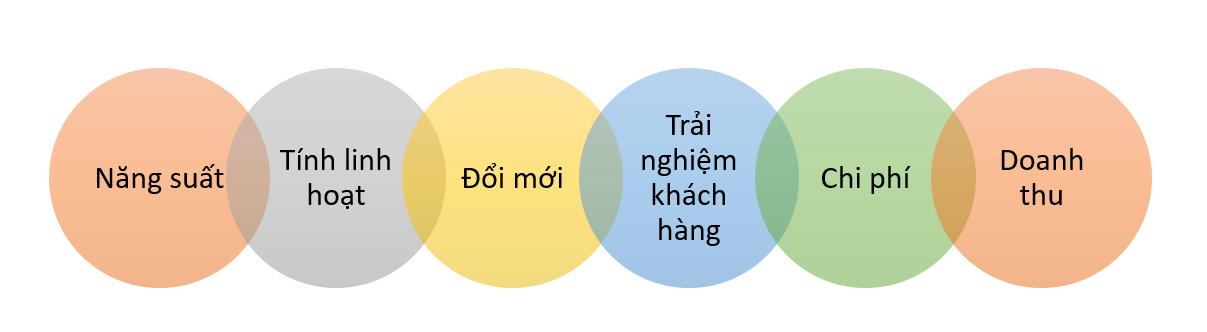
\includegraphics[width=\textwidth]{Images/Intro/advantage.jpg}
    \caption{Lợi ích của các công nghệ Công nghiệp 4.0}
    \label{fig:advantage}
\end{figure}

Với sự phát triển nhanh chóng của những công nghệ của nền Công nghiệp 4.0 đã được nêu ở trên và những ứng dụng mà nó mang lại, phương thức sản xuất của các doanh nghiệp sản xuất đang được chuyển từ kỹ thuật số sang thông minh (digital to intelligent). Kỷ nguyên mới của sự kết hợp công nghệ thực tế ảo dựa trên Hệ thống vật lý mạng (Cyber-Physical System) đang đến. Trước những thách thức mới, lợi thế của các ngành sản xuất truyền thống đang dần bị mai một. Do đó, công nghệ sản xuất thông minh (intelligent manufacturing technology) là một trong những lĩnh vực công nghệ cao được các nước công nghiệp phát triển đặc biệt chú trọng. Chiến lược Châu Âu 2020 (Europe 2020 strategy), Chiến lược Công nghiệp 4.0 (Industry 4.0 strategy) và Sản xuất Trung Quốc 2025 (China manufacturing 2025) đã được đề xuất. Hoa Kỳ đã từng bước đẩy nhanh tốc độ tái công nghiệp hóa và tái sản xuất. Sự chuyển đổi của sản xuất thông minh đã gây tò mò về tác động sâu sắc và lâu dài của nó đối với ngành sản xuất trong tương lai trên toàn thế giới.

Đặc biệt, trong bối cảnh sản xuất thông minh, các nhà máy đã trở nên linh hoạt hơn bao giờ hết trước sự hỗn loạn phức tạp của thị trường hiện đại. Các khái niệm hiện đại về hệ thống sản xuất đòi hỏi sự tích hợp theo chiều dọc và chiều ngang của tất cả những người tham gia vào quá trình sản xuất. Do đó, điều quan trọng nhất là thiết lập nhà máy thông minh (smart factory) để có thể đạt được sản xuất tiên tiến dựa trên công nghệ mạng (network technologie) và dữ liệu sản xuất (manufacturing data). Nhà máy thông minh là một giải pháp sản xuất linh hoạt và hiệu quả để đáp ứng nhu cầu của thị trường ngày nay, đồng thời nó đạt được sự tích hợp giữa các đối tác công nghiệp và phi công nghiệp khác nhau, những người xây dựng các tổ chức năng động và các tổ chức ảo.


\section{Nhà máy thông minh - Smart factory}

% Sự phát triển của ngành công nghiệp 4.0 đã tạo ra những bước phát triển vượt bật trong thời hiện đại, tạo ra vô số những hướng phát triển mới cho các ngành công nghiệp, hướng tới không chỉ khả năng tự động hóa (autonomous) mà còn phải thông minh (smart). Mạng kết nối vạn vật trong công nghiệp (Industrial Internet of Things - IIoT) đã mở đường cho sự kết nối của vô số các thiết bị, cảm biến (asset) trong môi trường công nghiệp, liên kết chúng với nhau và giao cho chúng khả năng giao tiếp (Communication); dữ liệu được tập trung nhiều và dày đặc, tạo thành Dữ liệu lớn (Big Data), được đem đi xử lý nhằm tạo ra những dữ liệu tổng hợp có ý nghĩa, qua đó mang lại rất nhiều lợi ích cho các doanh nghiệp để họ đánh giá được chất lượng sản xuất sản phẩm, cũng như khả năng phát hiện sớm các vấn đề trong sản xuất và bảo trì chủ động (active maintenance) giúp tiết kiệm rất nhiều tài nguyên, chi phí và thời gian. Ngành công nghiệp 4.0 đã tạo ra rất nhiều sự phát triển trong ngành công nghiệp, và trong đồ án này sẽ tập trung vào Smart Factory (nhà máy thông minh), một xu hướng phát triển của công nghiệp khá nổi trong thời gian gần đây. Sự phát triển của nhà máy thông minh dự kiến sẽ mang lại sự phát triển vượt bậc dành cho các công ti, giúp họ tạo ra những sản phẩm tuyệt với đáp ứng nhu cầu ngày càng cao của khách hàng trong thời đại mới, trong khi tiết kiệm tối đa chi phí, thời gian và đạt lợi nhuận cao nhờ sự kết hợp với IIoT và tận dụng dữ liệu đa dạng của IIoT để thực hiện phân tích cho công tác sản xuất trở nên hiệu quả hơn.

Dưới sự ảnh hưởng cuộc cách mạng công nghiệp 4.0 và sự ra đời, phát triển của vô số các công nghệ mới như IoT, IIoT, Cloud computing, Cyper-security, Big Data Analytics... như trình bày ở trên, đã dẫn đến sự thay đổi lớn cho xu hướng công nghiệp thời đại mới, chú trọng hơn vào dữ liệu, về sự kết nối và tính thông minh, các mô hình sản xuất thuộc nhiều lĩnh vực khác nhau đã có những bước thay đổi, phát triển để phù hợp hơn, mà trong đó không thể không kể đến là mô hình nhà máy thông minh (Smart Factory). Smart Factory là một mô hình sản xuất công nghiệp đánh dấu bước trưởng thành đột phá của sản xuất trong thời đại công nghiệp 4.0 so với thời kì 3.0 trước đó, đem lại định nghĩa mới về sản xuất tại nhà máy không chỉ đơn thuần là "tự động", mà còn phải "tự hành" và "thông minh". Để có thể xây dựng một mô hình Smart Factory, ta có thể áp dụng và kết hợp các công nghệ mới của thời đại 4.0 trên, và đảm bảo chúng cần được liên kết với nhau để tận dụng tối đa sức mạnh mà các công nghệ mang lại. Trong phạm vi đề tài, nhóm chỉ giới hạn tìm hiểu về ứng dụng của công nghệ IoT, cụ thể là IIoT (Industrial Internet of Things) trong bối cảnh nhà máy thông minh.

Phần tiếp theo, nhóm sẽ trình bày ba ý chính của smart factory: Khái niệm và lợi ích của smart factory, kiến trúc đề xuất của nhóm cho các ứng dụng Smart Factory dựa trên mô hình năm lớp của diễn giả Timothy Chou, và cuối cùng là những thách thức của ứng dụng smart factory trong lớp Connect - Một trong năm lớp của kiến trúc ứng dụng thời đại 4.0 thuộc phạm vi nghiên cứu của đồ án, qua đó nêu ra được những giải pháp đã và đang được áp dụng để xử lý vấn đề đó trong môi trường công nghiệp ngày nay. 

\subsection{Định nghĩa và lợi ích của Smart Factory}

Smart Factory (Nhà máy thông minh) là một cơ sở sản xuất được "số hóa" sử dụng các thiết bị, máy móc và hệ thống sản xuất kết nối với nhau nhằm liên tục thu thập thông tin và chia sẻ dữ liệu. Dữ liệu này được sử dụng để tạo ra những dự đoán nhằm cải thiện quá trình sản xuất và chỉ ra các vấn đề đang gặp phải trong tiến trình này. Đọc định nghĩa trên, ta có thể chỉ ra hai ý chính làm nên một Smart Factory, đó chính là "sự kết nối của tất cả thiết bị" và "dự đoán". Thật vậy, nói đến smart factory, không phải ý chỉ là nhà máy chỉ trang bị những máy móc hiện đại và tự động là đủ, bởi những cỗ máy "tự động" này đã xuất hiện từ lâu ở thời đại công nghiệp 3.0. Sự khác biệt giữa Smart factory trong thời đại công nghiệp 4.0 này chính là việc các máy móc thay vì độc lập với nhau, chúng sẽ thông minh hơn, biết kết nối, giao tiếp và chia sẻ thông tin, tạo thành một mạng lưới thông tin khổng lồ giữa các thiết bị trong nhà máy. Hơn nữa, với lượng dữ liệu khổng lồ như vậy, sẽ là cơ hội để ta thu thập và phân tích chúng - sử dụng trí tuệ nhân tạo để có thể thấy rõ những đặc trưng của sản xuất một cách thực tế, đồng thời giúp ta dự đoán những sự kiện mới, thậm chí là tạo ra những cải tiến cho mô hình sản xuất và truyền lại để các máy móc áp dụng. Smart Factory đã đề ra một nhà máy "kết nối" và "thông minh" hơn so với sự tự động hóa đơn thuần của các nhà máy thời đại công nghiệp 3.0

Khi áp dụng mô hình Smart Factory, doanh nghiệp sẽ nhận được nhiều lợi ích và ưu thế, đồng thời cải thiện hiệu năng sản xuất của mình. Một số lợi ích từ Smart Factory được liệt kê như sau:

\begin{itemize}
    \item \textbf{Tăng cường năng suất và hiệu quả}:  Trong suốt lịch sử, sự thành bại của sản xuất công nghiệp là từ sự phản ứng nhanh nhạy trước những sự kiện hay xu hướng đang xảy ra và cố gắng để dịch chuyển phương hướng sản xuất theo xu hướng đó. Nhưng với Smart Factory, ta có thể giảm bớt cơ chế phản ứng lỗi thời, tạo ra khả năng quản lý nguồn cung một cách linh hoạt và hợp lý hơn. Thật vậy, nhờ vào khả năng dự đoán phân tích (predictive analytics) và dữ liệu lớn (Big Data) khi áp dụng vào smart factory, giúp nhà máy có thể tìm ra được phương hướng sản xuất tối ưu và phù hợp với xu hướng hiện tại. Quản lý tài nguyên kịp thời (Just-in-time), dự đoán trước nhu cầu chính xác và tăng cường tốc độ sản xuất ra thị trường là các lợi ích có được từ smart factory, giúp tiết kiệm chi phí đồng thời tăng khả năng đáp ứng nhanh của doanh nghiệp trước sự thay đổi chóng mặt của thị trường thời đại mới. Chưa hết, nhờ vào việc thu thập dữ liệu của các máy móc và sự giao tiếp giữa chúng trong một mạng nhà máy thông minh, doanh nghiệp có thể phân tích và dự đoán trạng thái của máy móc, qua đó kịp thời sửa chữa khi cần, giảm thời gian chết trong sản xuất và cải thiện năng suất nhà máy.
    \item \textbf{Sự ổn định và an toàn}: Việc áp dụng smart factory sẽ giúp doanh nghiệp tìm ra được những phương pháp sản xuất "xanh", an toàn và có trách nhiệm với môi trường. Đồng thời, do dây chuyền sản xuất được tự động hóa một cách thông minh sẽ giúp tránh được lỗi sai của sản phẩm do con người, giúp tăng tính ổn định của sản phẩm và đảm bảo được chất lượng. Một sản phẩm được sản xuất từ việc áp dụng smart factory sẽ giúp khách hàng yên tâm sử dụng hơn và họ sẽ chấp nhận trả nhiều tiền hơn cho sản phẩm đó, góp phần vào việc tăng dần doanh thu của nhà máy.
    
\end{itemize}

\subsection{Kiến trúc của Smart Factory}

Trong thời đại công nghiệp 4.0, sản xuất thông minh (intelligent manufacturing) thu hút nhiều sự quan tâm từ nhà nước, các chuyên gia và các nhà nghiên cứu khoa học. Theo đó, sự xây dựng nên kiến trúc của Smart Factory cũng được nghiên cứu. Smart Factory là dựa trên phương hướng xây dựng nhà máy "số hóa" (digital) và "tự động" (automated), sử dụng công nghệ thông tin như nền tảng đám mây hoặc IIoT để cải thiện khả năng quản lý tài nguyên sản xuất và chất lượng dịch vụ. \cite{chen} Hiện tại, vẫn chưa có một hiện thực nào của Smart factory được chuẩn hóa và công bố, tuy nhiên, dựa theo nhiều nghiên cứu khác nhau, Chen et al. \cite{chen} cho rằng có ba lớp chính trong kiến trúc của Smart factory:
\begin{itemize}
    \item \textbf{Lớp vật lý}: gồm các thiết bị vật lý cần sự hỗ trợ để lấy được dữ liệu nhanh chóng trong thời gian thực, các thiết bị giao tiếp phải cung cấp khả năng truyền nhanh chóng, kể cả loại dữ liệu phức tạp.
    \item \textbf{Lớp mạng}: Lớp này quy định cách thức kết nối giữa các thiết bị vật lý và thu thập chúng tới các server edge để xử lý. Về phương thức kết nối, smart factory sử dụng Industrial Internet of Thing - IIoT. Với việc áp dụng IIoT, Các phương pháp để giao tiếp giữa các thiết bị trong nhà máy như Mạng cảm biến công nghiệp (Industrial Wireless Sensor Networks - IWSNs) cần được nghiên cứu.
    \item \textbf{Lớp dữ liệu} Dữ liệu thu thập được từ các thiết bị cần được tập hợp ở nền tảng đám mây, sau đó có khả năng phân tích tìm ra ngữ nghĩa của nhiều loại dữ liệu khác nhau, đặc biệt hơn hết là tạo ra khả năng tự tổ chức, tự học và tự áp dụng ở các thiết bị thông minh này nhằm cải thiện năng suất nhà máy. Đây là lớp áp dụng các công nghệ phân tích, trí tuệ nhân tạo nhằm tận dụng lượng dữ liệu khổng lồ thu thập được từ các thiết bị để đưa ra những dự đoán và tối ưu cho công tác sản xuất của smart factory
\end{itemize}

Có thể thấy, ba lớp kiến trúc được trình bày trên có những điểm tương đồng nhất định với kiến trúc năm lớp cho các ứng dụng thời đại 4.0 được đề xuất bởi diễn giả Timothy Chou: Lớp vật lý gồm "Things", lớp mạng gồm "Connect" và "Collect", và lớp dữ liệu bao gồm "Learn" và "Do". Mô hình năm lớp của diễn giả Chou có sự phân tách sâu hơn về chức năng của một ứng dụng 4.0, do đó sẽ được nhóm tập trung phân tích. Trong phạm vi của đề tài, nhóm sẽ chú trọng và lớp kết nối (Connect) trong ứng dụng thời đại 4.0 nói chung và trong kiến trúc ứng dụng smart factory nói riêng, nhằm có cái nhìn cụ thể hơn về các thức kết nối các thiết bị thông minh trong smart factory.

Ở phần tiếp theo, nhóm sẽ tập trung vào lớp kết nối này, nhằm nhìn nhận những thách thức trong việc hiện thực lớp kết nối cho ứng dụng smart factory và đề ra những giải pháp đang được áp dụng hiện nay để giải quyết những thách thức đó

% \begin{figure}[!h]
%     \centering
%     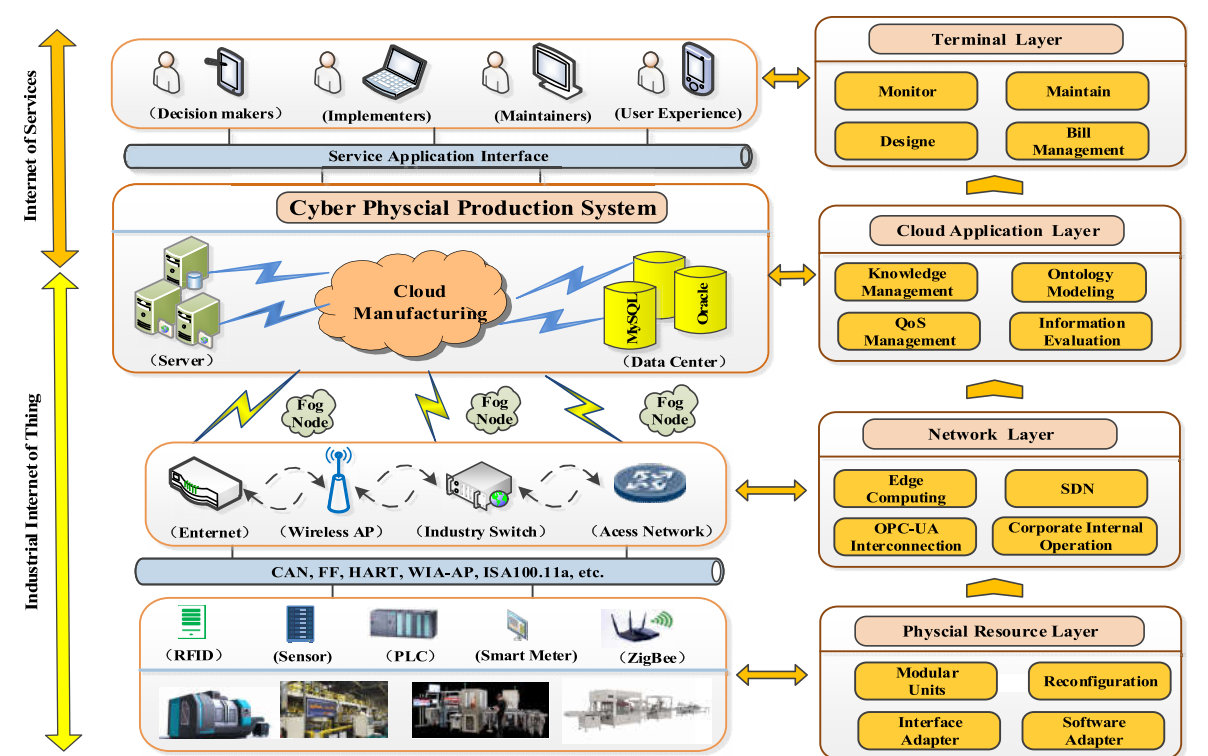
\includegraphics[width=\textwidth]{Images/Intro/sf_0.jpg}
%     \caption{Kiến trúc của nhà máy thông minh \cite{chen}}
%     \label{fig:sf_0}
% \end{figure}

\subsection{Thách thức của lớp kết nối}

% Việc áp dụng được Smart Factory là một thách thức không nhỏ đối với các doanh nghiệp, ảnh hưởng tới nhiều khía cạnh từ kĩ thuật cho tới kinh doanh, chưa kể, đây vẫn là một hình thức phát triển mới dành cho các nhà máy và vẫn chưa có một tiêu chuẩn cụ thể. Do đó, xây dựng smart factory sai cách có thể ảnh hưởng rất nhiều tới doanh nghiệp. Trong phần này, nội dung sẽ tập trung về triển khai Smart Factory về khía cạnh kĩ thuật, từ đó thấy được những khó khăn và thách thức cần được giải quyết khi hiện thực lớp kết nối cho ứng dụng Smart Factory. 
% \subsubsection{Lớp vật lý}

% Trong nhà máy thông minh, lớp vật lý này bao gồm toàn bộ tài nguyên vật lý liên quan tới suốt vòng đời sản xuất, nhưng chủ yếu chú trọng vào các thiết bị sản xuất thông minh trong nhà máy. Để đảm bảo sản xuất trở nên "thông minh" và "hiệu quả" hơn, những tiêu chí sau cần được chú trọng và giải quyết:
% \begin{enumerate}
%     \item \textbf{Các thành phần sản xuất theo dạng khối (Modular manufacturing units)}
    
%     Sẽ rất khó cho các doanh nghiệp sản xuất để linh hoạt trước sự thay đổi nếu chuỗi các thiết bị sản xuất dính liền với nhau. Thay vào đó, sử dụng các thiết bị sản xuất ở dạng đơn lẻ (khối), sau đó kết hợp với nhau để tạo thành một chuỗi sản xuất hoàn chỉnh, nhưng vẫn có khả năng tùy chỉnh, tách và chỉnh sửa lại kiến trúc khi cần. Điều này cần thiết có một nền tảng (framework) để quản lý sự kết hợp và sắp xếp các khối thiết bị này. Hơn nữa, các khối thiết bị cần phải tăng cường sự "thông minh" của bản thân chúng, tức, một khối thiết bị đảm nhận công việc phải có khả năng làm việc độc lập và tuân theo những thay đổi về lịch trình trong một nhà máy thông minh.
%     \item \textbf{Thiết bị điều khiển có thể điều chỉnh được (Configurable controller)}
    
%     Khả năng điều chỉnh được cho một hệ thống điều khiển tức là khả năng tích hợp, mở rộng, thay thế hoặc sử dụng lại phần cứng - phần mềm. Điều này áp dụng cho toàn bộ hệ thống sản xuất và cả những khối thiết bị sản xuất nhỏ, tạo nên sự linh hoạt trong sản xuất tại nhà máy. Điều này đồng nghĩa với việc các thiết bị sản xuất cần được phát triển kì công hơn, với nhiều tính năng hơn và chú trọng vào khả năng mở rộng, nâng cấp, tự sửa chửa, thay thế nhanh chóng.
%     \item \textbf{Dây chuyền sản xuất có thể tùy chỉnh được (Reconfigurable Production line)}
    
%     Ngày nay, sản phẩm được sản xuất trong thị trường thường ở dạng lô nhỏ nhưng đa dạng về loại hình, do đó, nhà máy thông minh cần phát triển khả năng tùy chỉnh dây chuyền sản xuất "thời gian thực", thay đổi loại sản phẩm sản xuất và số lượng sản xuất "thời gian thực". Điều này có khả năng tạo ra sự linh hoạt tuyệt vời, khi nhà máy có thể sản xuất ra nhiều loại sản phẩm khác nhau với số lượng khác nhau trong các khoảng thời gian khác nhau, chính nhờ vào khả năng tùy chỉnh, mở rộng và lập lịch trình hoạt động của dây chuyền sản xuất.
%     \item \textbf{Thu thập dữ liệu thông minh (Intelligent Data acquistion)}
    
%     Các thiết bị sản xuất giờ đây sẽ "thông minh" hơn, và mang trong mình nhiều loại dữ liệu phức tạp từ các cảm biến. Chính vì vậy, các thiết bị cần thiết phải hỗ trợ nhiều phương thức giao tiếp khác nhau như OPC, Open Database Connectivity (ODBC), RS232... để kết nối được vào các thiết bị kiểm soát như Supervisory Control and Data Acquisition (SCADA), Distributed Control System (DCS),... Thêm nữa, việc thu thập dữ liệu từ các thiết bị cần phải dễ dàng để cài đặt, các cổng giao tiếp linh hoạt và dễ mở rộng. Đặc biệt, thông tin về tình trạng của thiết bị cũng cần được cung cấp để quan sát, theo dõi nhằm bảo trì, thay thế sớm khi cần thiết.
% \end{enumerate}

% \subsubsection{Lớp mạng}

Trong lớp kết nối này là lớp tập trung vào vấn đề kết nối giữa các thiết bị với nhau. Trong nhà máy, công nghệ kết nối thường dùng có thể là dây bus (field bus) hoặc mạng cảm biến (sensor network). Do sự phát triển nhanh chóng của điện toán đám mây, để truyền tải dữ liệu, nhà máy thông minh yêu cầu một công nghệ mạng có thể truyền tải thời gian thực (real-time) và đáng tin cậy, nhằm chia sẻ dữ liệu giữa các thiết bị thông minh với nhau và nền tảng đám mây. Ta có thể sử dụng các dây truyền dẫn trực tiếp nhằm đảm bảo về tốc độ truyền và sự toàn vẹn dữ liệu, tuy nhiên áp dụng nó trong tình huống nhà máy lớn với vô số các cảm biến và thiết bị sẽ tăng độ phức tạp, cản trở sự mở rộng và linh hoạt ứng biến của nhà máy. Do đó, lớp mạng cần được thiết kế để đảm bảo sự linh hoạt, tiện lợi, dễ sử dụng. Mạng cảm biến không dây công nghiệp (Industrial Wireless Sensor Networks - IWSNs) đang được áp dụng nhiều cho các nhà máy thông minh hiện nay để đảm bảo tính kết nối linh hoạt của nhà máy, tuy nhiên chính từ phương thức xây dụng lớp kết nối này cũng tạo ra nhiều thách thức không nhỏ.

\begin{figure}[!h]
    \centering
    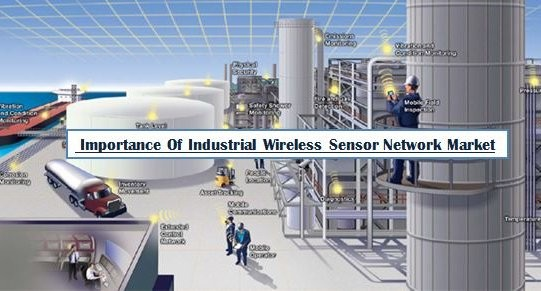
\includegraphics[width=\textwidth]{Images/Intro/sf_2.jpg}
    \caption{Mạng cảm biến không dây công nghiệp, từ \cite{wsnweb}}
    \label{fig:sf_2}
\end{figure}

Một số thách thức từ việc xây dựng mạng cảm biến không dây công nghiệp cho lớp kết nối có thể được kể đến như:

\begin{itemize}

    
   \item Mạng cảm biến không dây công nghiệp xuất hiện và phổ biến là nhờ sự phát triển và mở rộng vượt bậc của các công nghệ giao tiếp không dây trong thời đại hiện nay, và các công nghệ dành riêng cho công nghiệp. Việc triển khai mạng cho công nghiệp đã dần trở nên linh hoạt, và ít chi phí hơn, tuy nhiên, vì ứng dụng mạng trong công nghiệp vẫn rất phức tạp, nên hiện chưa có một chuẩn giao tiếp không dây tổng quát nào.
    
   \item Yêu cầu của mạng không dây trong công nghiệp trong bối cảnh nhà máy thông minh bắt buộc phải có độ trễ thấp, độ tin cậy cao, độ đồng bộ chính xác khi xử lý các dịch vụ điều khiển, khả năng chịu tải truy cập tốt và tiêu tốn năng lượng thấp khi thu thập dữ liệu. Trong đó, độ tin cậy và độ trễ của dữ liệu là yêu cầu quan trọng nhất trong việc xây dựng mạng không dây cho nhà máy thông minh, bởi dữ liệu là nền tảng cho công việc sản xuất và vận hành của nhà máy. Đôi khi, truyền tải dữ liệu bị mất đồng bộ với xung clock có thể gây mất gói, trì hoãn.
    
    \item Yếu tố đáng quan tâm nữa dành cho mạng không dây công nghiệp là bảo mật. Vì mạng không dây sử dụng các sóng radio, nên chúng dễ dàng bị xâm phạm bởi cả những người dùng không được ủy quyền, dễ tổn hại hơn so với hệ thống mạng dùng dây. Những cuộc tấn công mạng không dây vào nhà máy có thể gây ra tổn hại nghiêm trọng tới khả năng sản xuất của nhà máy. Hơn nữa, mạng không dây cũng không thể áp dụng các giải thuật bảo mật đang được dùng rộng rãi bên ngoài do chịu giới hạn về vấn đề năng lượng và sức mạnh tính toán hay tài nguyên mạng. Việc xây dựng một cơ chế bảo mật cho mạng không dây công nghiệp vẫn là một vấn đề nan giải cho đến ngày nay.

\end{itemize}

    Một số công nghệ đã được sử dụng để giải quyết vấn đề trong lớp kết nối sử dụng mạng không dây tại nhà máy, các chuẩn không dây như NB-IoT, 5G, LTE, 3GPP cung cấp khả năng giao tiếp không dây với độ trễ thấp và độ tin cậy cao. 
    % Các giao thức M2M (machine to machine) thông dụng như MQTT, OPC-UA cũng được xem xét áp dụng. MQTT thường được dùng để truyền tải dữ liệu gọn nhẹ và tiết kiệm năng lượng, là một giao thức phổ biến trong IoT. 
    Giao thức OPC-UA - một giao thức dạng M2M (Machine to Machine) cũng được dùng nhiều trong môi trường công nghiệp, như một giải pháp để truyền tải dữ liệu có cấu trúc với tốc độ cao và đáng tin cậy, được phát triển theo hướng tập trung vào dịch vụ (service oriented). OPC-UA là một giao thức đa nền tảng, phù hợp cho nhiều loại hệ điều hành, cộng với khả năng bảo mật tốt, cho phép giao tiếp hiệu quả giữa các khối thông minh với nhau trong môi trường nhà máy. 

    Trong đề tài này, nhóm sẽ chủ yếu tập trung vào giao thức được dùng rộng rãi trong ngành công nghiệp hiện nay, và được hỗ trợ bởi đa số các thiết bị phần cứng hiện đại trong nhà máy là giao thức OPC-UA, một giao thức chuẩn công nghiệp theo hướng dịch vụ, được phát triển với mong đợi giải quyết các vấn đề hóc búa về giao tiếp giữa các thiết bị thông minh trong nhà máy với tốc độ cao, độ ổn định tốt và đáng tin cậy về dữ liệu.


% \subsubsection{Lớp dữ liệu ứng dụng}

% Các thiết bị cung cấp dữ liệu ở tầng vật lý, được vận chuyển bởi tầng mạng, và các dữ liệu thu thập được sẽ được xử lý ở lớp dữ liệu. Xử lý dữ liệu là một thao tác quan trọng trong nhà máy thông minh, bởi sẽ vô nghĩa nếu ta thu thập dữ liệu nhưng không thể xử lý và tận dụng thông tin từ chúng. Ở bước này, ta cần phương pháp xử lý dữ liệu hợp lý, bởi dữ liệu trong nhà máy tới từ nhiều thiết bị với nhiều định dạng khác nhau, tạo nên sự phức tạp của dữ liệu. Phương hướng phân tích dữ liệu cũng là một vấn đề đau đầu cho các chuyên gia nhằm trích xuất ra các đặc điểm và kết luận đúng đắn, chưa kể là có khả năng dữ liệu bị lỗi do nhiễu hoặc các yếu tố môi trường. 

% Mục đích xây dựng lớp dữ liệu nhằm để tạo nên phương hướng phát triển "dựa vào kiến thức" (knowledge-driven manufacturing). Điều này tạo ra nhiều cơ hội để thay đổi phương hướng sản xuất truyền thống trở thành công nghiệp thông minh, cho phép nhìn nhận khả năng sản xuất của nhà máy, chất lượng sản phẩm, thiết bị và nhiều yếu tố khác. Phân tích dữ liệu tốt có thể tạo ra khả năng bảo trì chủ động (active maintenance) nhờ vào quan sát sức khỏe của các thiết bị để thông báo sớm các vấn đề xảy ra và xử lý kịp thời để giảm thời gian chết trong sản xuất, tránh làm trì trệ sản xuất. Mặt khác, thông qua phân tích dữ liệu, ta có thể tìm ra phương hướng tối ưu sản phẩm, tối ưu dây chuyền sản xuất cho nhà máy thông minh. Chưa kể, khả năng tự học, tự tìm ra phương pháp tối ưu và tự áp dụng nó lên quy trình sản xuất được thực hiện bởi các thiết bị hiện đại và phần mềm xử lý sẽ tạo ra sự đột phá trong chất lượng sản xuất nhà máy.


% Trong ba lớp của kiến trúc nhà máy thông minh, đề tài này có phạm vi tập trung vào lớp mạng, nhằm nghiên cứu giao thức OPC-UA, một giao thức chuẩn công nghiệp được sử dụng rộng rãi trong các nhà máy, nhằm đánh giá ưu, nhược, xem xét khả năng của nó trong việc giải quyết các vấn đề còn tồn đọng của nhà máy thông minh và phương hướng sử dụng OPC-UA trong ứng dụng công nghiệp - điều khiển các thiết bị trong nhà máy.

% Để vượt qua những khó khăn này, trong mỗi chương, chúng em sẽ phân tích và đưa ra những hướng giải quyết phù hợp. Ở phần kết luận, chúng em sẽ tóm tắt toàn bộ các vấn đề và đề xuất công việc trong tương lai cho những khó khăn chưa được giải quyết.


\section{Giới thiệu về Đồ Án}

Trong những năm gần đây, sự phát triển của giao tiếp Machine-to-Machine (M2M) và Internet of Things (IoT) trong Công nghiệp đã mở đường cho việc phát triển các máy móc thông minh và điều khiển tự động trong các doanh nghiệp sản xuất. Các máy tự động này có khả năng thu thập dữ liệu từ các thiết bị cảm biến khác nhau và giao tiếp với các hệ thống máy được kết nối khác bằng cách sử dụng các giao thức truyền thông. Điều này được thể hiện rõ nét nhất qua Lớp Connect theo như mô hình năm lớp của Timothy Chou đã được trình bày ở phần trên. Và để đảm bảo được việc các thiết bị có thể trao đổi thông tin với nhau có hiệu quả cao nhất về sự chính xác, và đồng bộ nhanh, đặc biệt là trong môi trường Công nghiệp - Smart Factory, thì việc lựa chọn ra một giao thức kết nối an toàn và phù hợp là điều vô cùng quan trọng. Vì thế, nội dung nghiên cứu của Đồ án này cũng sẽ tập trung vào Lớp Connect, lớp tạo nên kết nối vạn vật giữa các thiết bị - và cụ thể hơn là nghiên cứu và hiện thực một giao thức truyền thông chuyên dụng trong Công nghiệp hiện nay - \textbf{OPC-UA}. 

% Theo như kiến trúc 5 lớp của Timothy Chou đã được mô tả ở phần đầu, thì trong phạm vị của Đồ án này, nôi dụng nghiên cứu sẽ chỉ tập trung vào lớp Connect, lớp tạo nên kết nối vạn vật giữa các thiết bị. Và để đảm bảo được việc các thiết bị có thể trao đổi thông tin với nhau có hiệu quả cao nhất về sự chính xác, và đồng bộ nhanh, đặc biệt là trong môi trường Công nghiệp - Smart Factory, thì việc lựa chọn ra một giao thức kết nối an toàn và phù hợp là điều vô cùng quan trọng. Do đó, các giao thức truyền thông đặc trưng trong thời đại Công nghiệp 4.0 sẽ được so sánh, nghiên cứu và hiện thực trong Đồ án này. Nội dung nghiên cứu tổng quan gồm những vấn đề chính sau:
Nội dung nghiên cứu tổng quan gồm những vấn đề chính sau:
\begin{itemize}
    \item \textbf{Các giao thức chuyên dụng cho Smart Factory}\\
    	Trong nội dung nghiên cứu này, hai giao thức truyền thông thông dụng M2M (MQTT và OPC-UA) sẽ được phân tích để phân biệt rõ ưu điểm và nhược điểm của chúng. Bên cạnh đó, một số thí nghiệm sẽ được thực hiện, chúng em sẽ xây dựng hai kiến trúc tương đương nhau cho các giao thức OPC UA và MQTT rồi tiến tới so sánh hiệu năng của chúng dựa trên việc so sánh Round Trip Time (RTT) của hai giao thức, qua đó đánh giá được tốc độ gửi nhận của gói tin trong một số tình huống. Từ đó, có thể nhận thấy được giao thức nào chiếm ưu thế và phù hợp hơn trong môi trường Công nghiệp.
    \item \textbf{Thiết kế kiến trúc, Hiện thực điều khiển cánh tay Robot dựa trên OPC-UA và phát triển ứng dụng digital twin}\\
    	Và cuối cùng, để kiểm nghiệm hiệu quả của giao thức OPC-UA, chúng em sẽ thiết kế một hệ thống, kết nối một số thiết bị thông dụng (Cánh tay Robot JetMax, Ứng dụng VR điều khiển cánh tay...) với nhau thông qua giao thức OPC-UA và xây dựng một ứng dụng digital twin để minh họa cho một số hoạt động cơ bản trong công nghiệp.

    
\end{itemize}

\section{Bố cục của đồ án}

Phần tiếp theo của Đồ án sẽ được chia thành 4 chương: Ở chương 2 sẽ giới thiệu tổng quan về các loại giao thức M2M (MQTT và OPC-UA) cũng như các công nghệ được nghiên cứu và sử dụng trong Đồ án. Chương 3 sẽ tiến hành thiết kế kiến trúc hệ thống và hiện thực điều khiển cánh tay Robot bằng giao thức OPC-UA. Chương 4 là phần đánh giá kết quả Đồ án mà nhóm đã làm được. Và cuối cùng là chương 5, tổng kết và đề ra những định hướng có thể phát triển trong tương lai.
